\setchapterimage[8.5cm]{tde}
\setchapterpreamble[u]{\margintoc}
\chapter{Stacking Analyses with IceCube}
\labch{results}
\begin{fquote}[Winston Churchill][Lady Windermere's Fan][18??]...man will occasionally stumble over the truth, but usually manages to pick himself up, walk over or around it, and carry on. 
\end{fquote}


What did we see? Excellent question...

\section{TDEs}

\subsection{Catalogues}

Four distinct TDE catalogues were compiled as part of this analysis, using data from the OpenTDECatalog CITE, as well as data from the literature and public data from CRTS/ASASSN. From the starting point of all TDEs, two subsamples were created:

\begin{itemize}
	\item \textbf{Jetted TDEs} are X-Ray-bright TDEs which launched relativistic jets pointing towards the Earth. There are three jetted TDEs, and neutrino emission is most promising from this category
	
	\item \textbf{Obscured TDEs} are TDE candidates which occur in very dusty galaxies, and are only observed via reprocessed infra-red emission. It is unclear whether these objects are actually TDEs, with Changing-Look Active Galactic Nucleii (CLAGN) being one alternative explanation. Depending on the galaxy geometry, there would be a delay of unknown length between maximal TDE luminosity and the detected peak IR luminosity. The search window for neutrino emission from obscured TDEs is consequently much less constrained.
\end{itemize}
Of the remaining TDEs, attention was paid to the possibility of source confusion. To avoid contamination of the catalogue by missclassified AGN or SN, the remaining TDEs were further split into a golden sample of reliably-classified TDEs, and those with more ambiguous classification.
\begin{itemize}
	\item \textbf{Golden TDEs} are strong candidates where the TDE interpretation is supported by multiple spectra
	\item \textbf{Silver TDEs} are all other candidates, where a TDE interpretation is either likely or not disfavoured.
\end{itemize}

For each jetted/gold/silver TDE, an individual search window was defined for neutrino emission, according to the following criteria:

\begin{itemize}
	\item For TDEs in which the light curve was observed when rising, the first measurement is taken as the window start.
	
	\item For TDEs without an observation during lightcurve rise, the last upper limit is taken as the window start.
	
	\item The maximum date was taken as the date on which the brightest TDE luminosity measurement was performed.
	
	\item The window extends from the defined window start to 100 days after the maximum date
	
\end{itemize}

Applying these criteria gives a tailored search window for each TDE. To account for potential delay following neutrino emission, Obscured TDEs instead had a search window extending from 300 days before peak to 100 days after peak. The four catalogues, including search windows, are provided in the Appendix. It is the first such catalogue to contain time windows, and could be used for stacking analyses of e.g gamma-ray emission.

In addition, four TDEs were selected for individual analysis. Two of the three jetted TDEs, Swift J1644+57 and Swift J2058+05, were chosen due to their luminosity, as well as their position in the northern hemisphere where IceCube has the highest effective area. In addition, ASSASN-14li and  XMMSL1 J0740-85 were chosen as non-jetted TDEs which were both nearby and bright. These four TDEs were the only catalogue sources that were also detected in radio observations, typically a tracer for relativistic particle acceleration.

For each of the four individual TDEs, searches were conducted for neutrino clustering in both time and space (see e.g \cite{IceCube:2018cha}). With the spatial and energy PDFs, all 'significant' neutrinos with $\frac{\mathcal{S}}{\mathcal{B}} \geq 1$ were identified. For each unique neutrino pair, a likelihood ratio test was performed as above assuming a uniform neutrino lightcurve between the pair arrival times. To account for the higher number of possible pairs with short periods relative to longer ones, a marginalisation term is introduced and the test statistic is defined as:

\begin{equation*}
	\lambda = 2\times \log \left( \frac{\mathcal{L}(\hat{n}_\text{s}, \hat{\gamma})}{\mathcal{L}(0)} \frac{T_{pair}}{T_{window}}\right)
\end{equation*}

where $T_{pair}$ is the detector livetime between the two neutrino arrival times, and $T_{window}$ is the search window length in detector livetime.

Of all tested pairs, that with the largest TS value is selected as the 'neutrino flare'. The significance of a TS value is again calculated from background-scrambled TS distributions. As can be seen in Figure \ref{fig:DiscTime}, for a short neutrino flare lying within a larger search window, the threshold neutrino fluence for discovery is significantly lower than with a traditional time-integration method.

All stacking tests are described in Table \ref{tab:stacking_tests}, and all single-object tests are described in Table \ref{tab:single_tests}.

\begin{table*}[]
	\centering
	\begin{tabular}{||c c c c | c||} 
		\hline
		Catalogue & Source Class & Size & Description  & Pre-trial p-value\\ [0.5ex] 
		\hline\hline
		Jetted & Jetted TDEs &  3 & \textit{Probable TDEs with on-axis jets} & 0.44\\ 
		\hline
		Golden & Non-Jetted TDEs & 13 & \textit{Probable TDEs with convincing classification}&1.0\\
		\hline
		Silver & Non-Jetted TDEs & 24 & \textit{Candidate TDEs with ambiguous classification}&1.0\\
		\hline
		Obscured & Non-Jetted TDEs & 13 & \textit{Candidate TDEs in dusty galaxies}&0.07\\[1ex] 
		\hline
	\end{tabular}
	\caption{Summary of the four TDE catalogues. For each, an independent stacking analysis was performed. The catalogues covered sources from May 2008 to October 2017, matching the IceCube data-taking period.}
	\label{tab:stacking_tests}
\end{table*}{}

\begin{table*}[]
	\centering
	\begin{tabular}{||c c c| c |} 
		\hline
		Object & Stacking Catalogue &  Isotropic-Equivalent Energy (ergs) & Pre-trial p-value\\ [0.5ex] 
		\hline\hline
		Swift J1655+57 & Jetted TDEs & $<2 \times 10^{54}$ & 1.0\\ 
		\hline
		Swift J2058+05 & Jetted TDEs & $<2 \times 10^{51}$& 0.38\\
		\hline
		ASASSN-14li & Non-jetted TDEs (Gold) & $<2 \times 10^{51}$& 1.0\\
		\hline
		XMMSL1 J0740-85 & Non-jetted TDEs (Gold)& $<2 \times 10^{51}$ & 0.22\\
		\hline
		\hline
		AT2018cow & - & $<2 \times 10^{51}$& ??\\
		[1ex] 
		\hline
	\end{tabular}
	\caption{Summary of the five individual TDEs for which the temporal-cluster-search method was applied. All but AT2018cow were included in the stacking analysis.}
	\label{tab:single_tests}
\end{table*}{}

Final p-values for each TDE catalogue, as well the four individual TDEs, are sumarised in Table A. The most significant result was obtained for Z. All values are consistent with those expected from background fluctuations, so no discovery is claimed. Instead we place upper limits on neutrino fluence from each catalogue and source. This is done in Figures \ref{fig:gold_flux} and \ref{fig:jetted_flux}  as a function of spectral index.

\begin{figure}[!ht]
	\centering 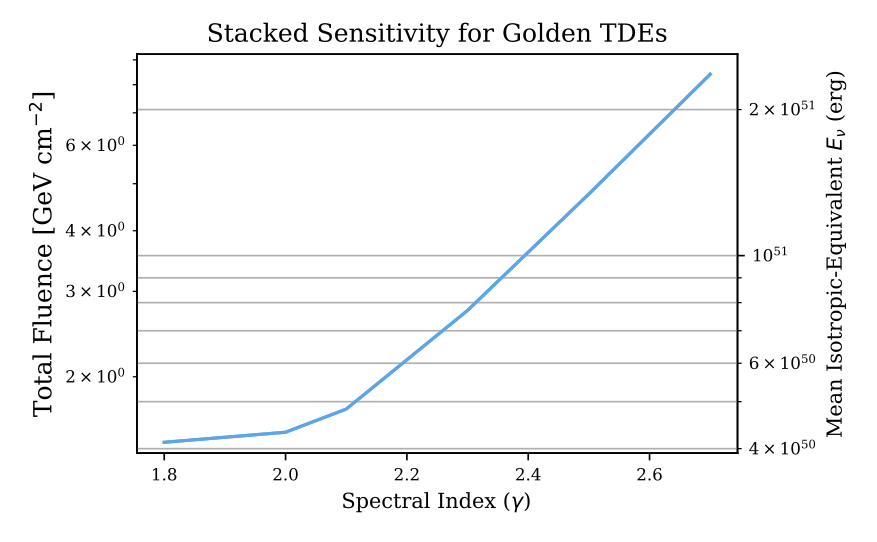
\includegraphics{results/gold_flux}
	\caption{Limits on the neutrino energy emitted by non-jetted TDEs as a function of spectral index, under the assumption of an unbroken power law between 100 GeV and 10 PeV. This limit is derived using the golden TDE sample, under the assumption that non-jetted TDEs are neutrino standard candles and emit isotropically.}
	\label{fig:gold_flux}
\end{figure}

\begin{figure}[!ht]
	\centering 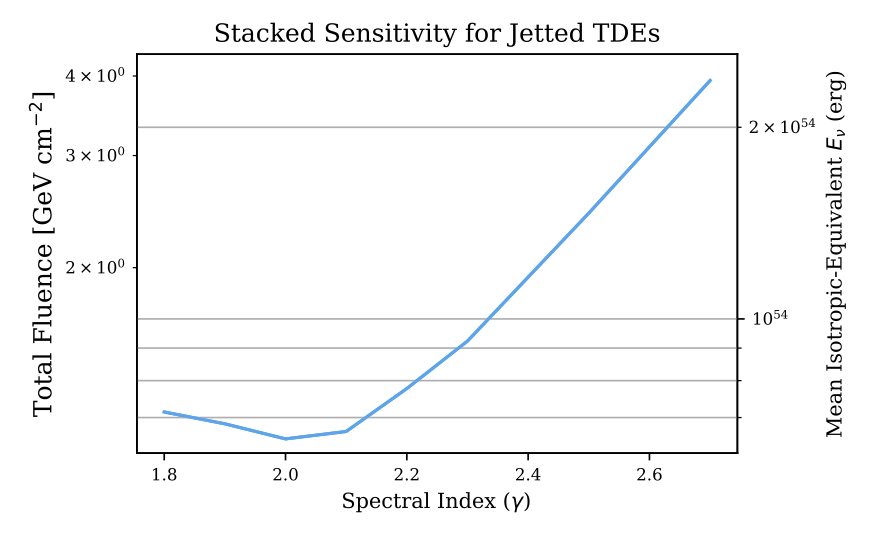
\includegraphics{results/jetted_flux}
	\caption{Limits on the isotropic-equivalent neutrino energy emitted by jetted TDEs as a function of spectral index, under the assumption of an unbroken power law between 100 GeV and 10 PeV. This limit is derived under the assumption that jetted TDEs are neutrino standard candles.}
	\label{fig:jetted_flux}
\end{figure}

As the likelihood tests made no assumptions for the relative brightness of each source, our results can be used to constrain a variety of emission distributions. Under the simplest assumption, we assume that each TDE is an equally neutrino-bright standard candle, and thus their contribution to the neutrino flux on Earth is simply proportional to $\frac{1}{D_{L}(Z)^{2}}$. 

As the Golden catalogue candidates were selected based on their strong likelihood of being genuine TDEs, the corresponding limits derived for the entire non-jetted TDE population can be considered robust. However, given the likely sample contamination, we do not attempt to similarly extrapolate results from silver or obscured samples to non-jetted TDEs as a population.

\subsection{Diffuse Neutrino Flux}

From the per-source limits derived in Figures \ref{fig:gold_flux} and \ref{fig:jetted_flux}, we can derive limits on the cumulative neutrino emission from non-jetted and jetted TDEs as populations. To do this, we calculate the rate of TDEs as a function of redshift, assuming a local rate and a source evolution derived in y. We then numerically integrate the flux contributed by shells of increasing redshift up to a horizon of z=8, to calculate the cumulative flux expected for each population. This method thus accounts for TDEs that were not detected by other surveys, and were therefore not incorporated into our catalogue.

To perform this calculation, we use the most recent IceCube global fit of the astrophysical neutrino flux, with a best-fit spectrum of $E^{-2.50}$ and normalisation of X at 100 TeV. For non-jetted TDEs, we assume a central local rate of $8 \times 10^{-7}$ Mpc$^{-3}$ year$^{-1}$ \sidecite{2018ApJ...852...72V}, a source evolution derived by \cite{Sun:2015bda}, and constrain the contribution of TDEs to be less than 26\% of the total. For jetted TDEs, under the assumption that they follow the same underlying source evolution as non-jetted TDEs with a central rate of $3 \times 10^{-11}$ Mpc$^{-3}$ year$^{-1}$ \sidecite{Sun:2015bda}, we find that they must contribute less than 1\% of the total.  These constraints are illustrated in Figure \ref{fig:DiffuseFlux}.

\begin{figure}[!ht]
	\centering 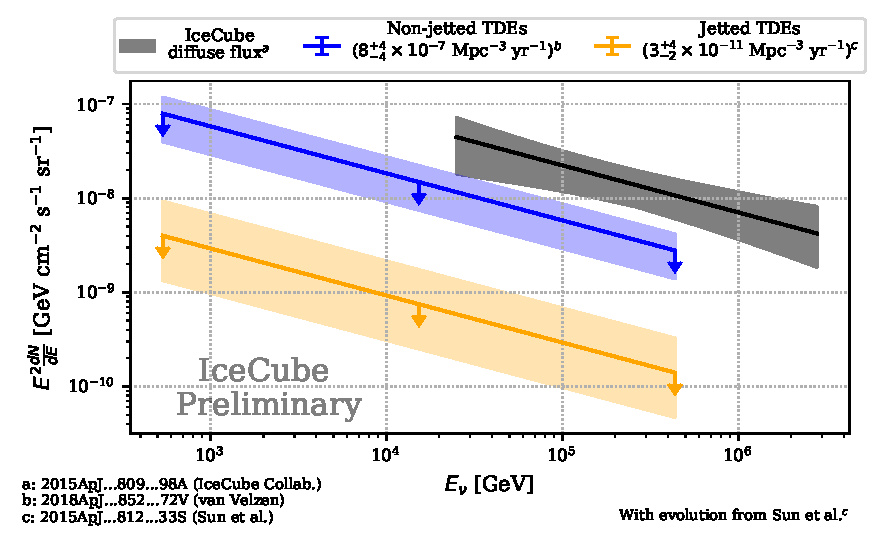
\includegraphics{results/tde_limits}
	\caption{Limits on the contribution of jetted and non-jetted TDEs to the diffuse neutrino flux, assuming standard candle behaviour. The shaded bands represent uncertainty in local rate estimates.}
	\label{fig:DiffuseFlux}
\end{figure}

As the contribution from a population is directly proportional to the local population rate, the shaded bands indicate the uncertainty in our limits arising from rate estimates. For TDEs, these rates are the dominant source of uncertainty in neutrino flux. It will require systematic evaluation of observed TDE rates to enable more precise limits on neutrino emission. Any refined rate estimate can be used to linearly rescale these limits. Propagating through the current local rate uncertainty, we constrain non-jetted TDEs to be less than 13-39\%, and jetted TDEs to be less than 0.n-1.n\% of the total.

\subsection{Limits}

\subsection{Individual Limits}



\section{AT2018cow and FBOTs}

Following the four stacking analyses and four object analyses described in Chapter \ref{ch:llh}, an additional analysis was performed on AT2018cow. This object
was a fast, bright, blue transient first discovered in 2018 cite. The observations suggested AT2018cow was a nearby example of a recently-identified population of Fast Blue Optical Transients (FBOTs) \sidecite{Margutti:2018rri}. 

Shortly after the time of discovery, AT2018cow was thought to be a Broad-Lined type IC (IC-BL) supernova, and thus a member of the rare CCSN subclass associated with long GRBs and choked-jets CITE. As many models predict that such SNe may be neutrino sources, an IceCube Fast Reponse Analysis was run on AT2018cow shortly after discovery CITE. Within the context of a candidate choked-jet supernova, the IceCube search focussed on the period spanning the 3-day period from the last non-detection to the first detection, aiming to isolate the supernova explosion time at which the neutrino emission would be expected. Ultimately, an excess of neutrinos was found in this time period, with a significance of 1.8 $\sigma$ \sidecite{2018ATel11785....1B}. The excess itself consisted of two signal-like neutrinos, which were considered significant owing to the small expected background for such a short search window.

Later multi-wavelength observations of AT2018cow were not consistent with a traditional IC-BL SN, and the transient has since variously interpreted as a TDE, an extreme SN or a Magnetar \sidecite{Perley:2018oky}. In light of these developments, AT2018cow was re-analysed by IceCube in the context of a potential TDE classification. As for the other four individual TDEs, a dedicated search for neutrino clustering on timescales up to 130 days, extending from 30 days before peak to 100 days afterwards, was undertaken.  For this purpose, an additional year of IceCube data extending to October 2018 was analysed.

In this analysis of AT2018cow, a small excess was again found. Although the best-fit cluster from this search included the two signal-like neutrinos from the original IceCube analysis, when accounting for the expected fluctuations arising from background over the much longer 130 day search window, the significance of the excess was just 0.5 $\sigma$. The results are thus entirely consistent with expectations from atmospheric background, while not contradicting the original result published at the time. As such, no discovery is claimed and upper limits are accordingly derived (illustrated in Figure \ref{fig:at2018cow_limits}). We emphasize that AT2018cow was not included in our catalogues at the time when the stacking analysis was performed, but would naturally belong to the silver non-jetted TDE sample. This object will be included in a future analysis incorporating more years of IceCube data.

\begin{figure}[!ht]
	\centering 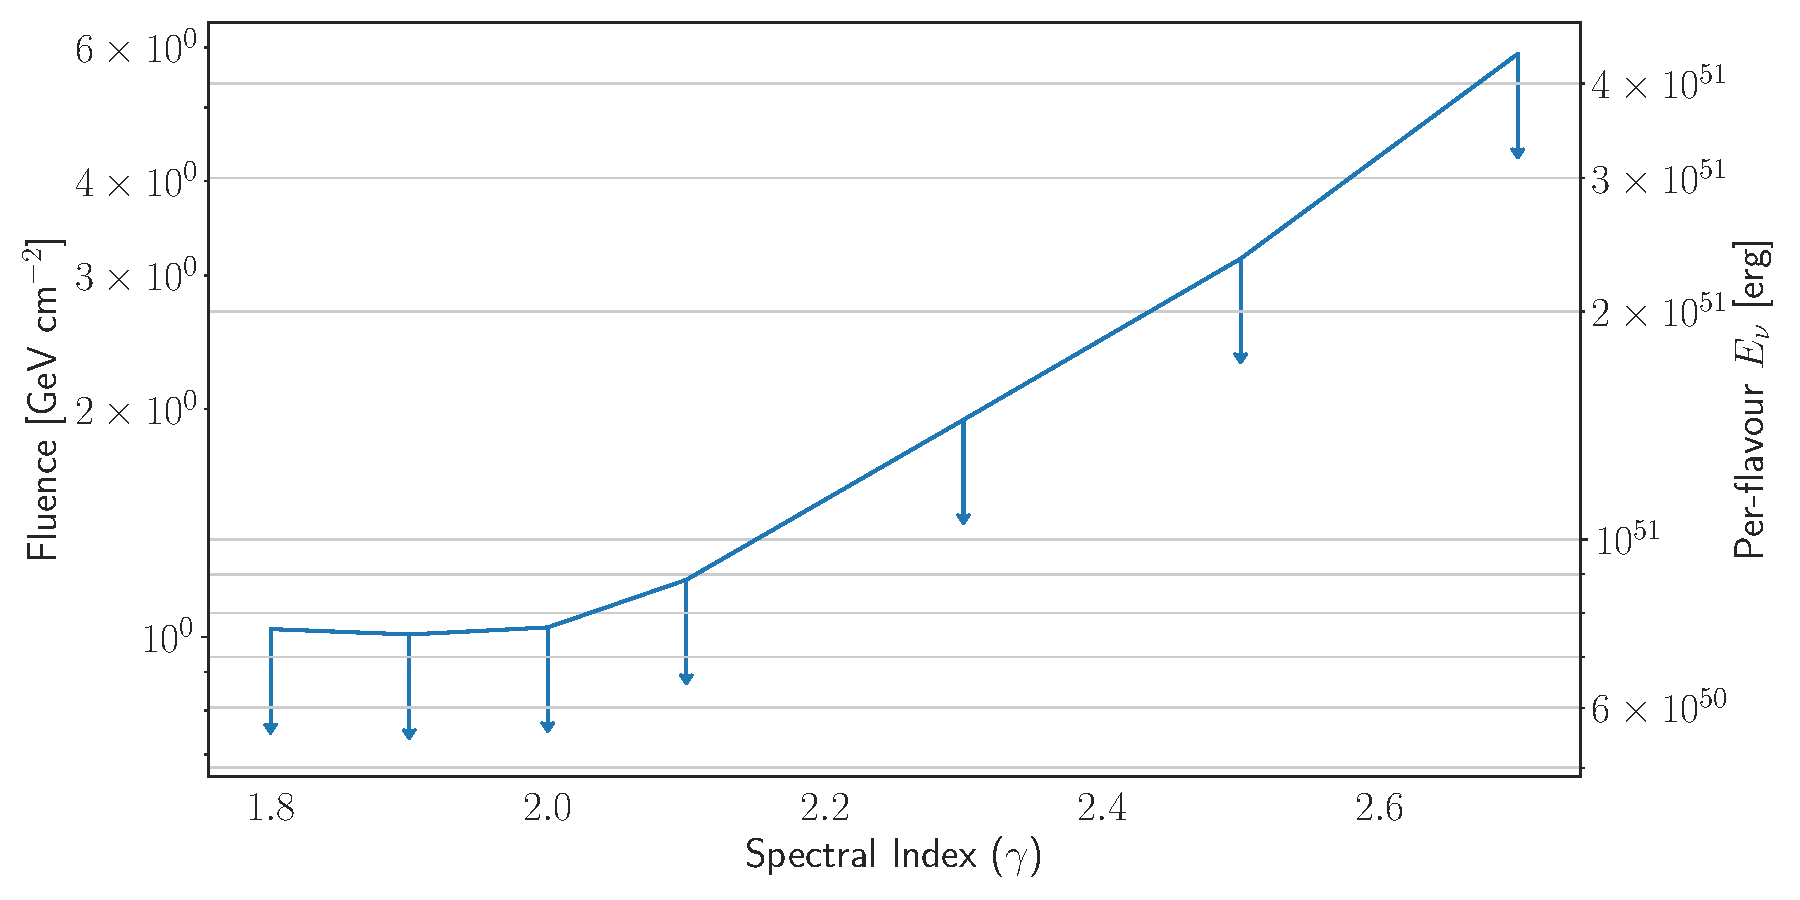
\includegraphics{results/at2018cow_limits}
	\caption{Limits on neutrino emission from AT2018cow, as a function of spectral index.}
	\label{fig:at2018cow_limits}
\end{figure}

\begin{figure}[!ht]
	\centering 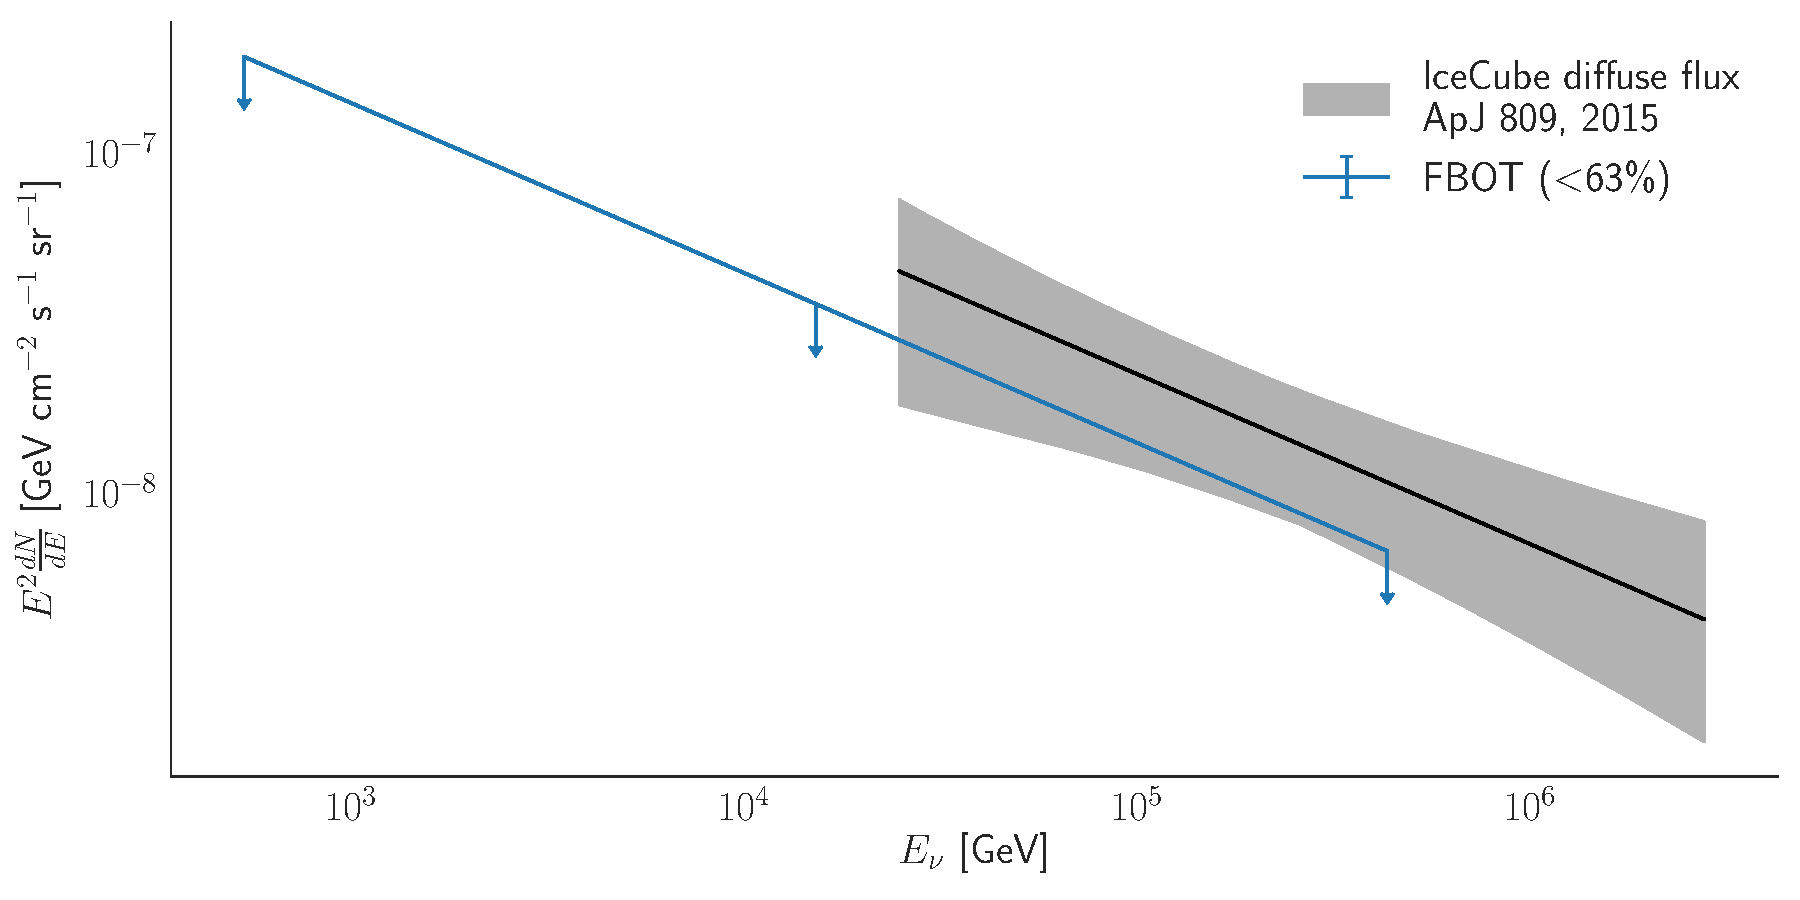
\includegraphics{results/fbot_limits}
	\caption{Limits on neutrino emission from from FBOTs, using the limits from AT2018cow under the assumption of neutrino standard candles.}
	\label{fig:fbot_limits}
\end{figure}